\documentclass[12pt, french]{article}

\usepackage{fancyhdr, fancybox, lastpage,mhchem}
\usepackage[most]{tcolorbox}
\usepackage[a4paper, margin={0.3in, .75in}]{geometry}
\usepackage{wrapfig}
\pagestyle{fancy}
\renewcommand\headrulewidth{1pt}
\renewcommand\footrulewidth{1pt}
\fancyhf{}
\rhead{ \em{Zakaria Haouzan}}
\lhead[C]{\em{2ème année baccalauréat Sciences Mathématiques}}
\chead[C]{}
\rfoot[C]{}
\lfoot[R]{}
\cfoot[]{\em{Page \thepage / \pageref{LastPage}}}


\newtcolorbox{Box2}[2][
enhanced,
breakable,
]{
                lower separated=false,
                colback=white,
colframe=white!20!black,fonttitle=\bfseries,
colbacktitle=white!30!gray,
coltitle=black,
enhanced,
attach boxed title to top left={yshift=-0.1in,xshift=0.15in},
title=#2,#1}


\begin{document}
\begin{center}
   \shadowbox {\bf{Les transformations liée a
des réactions acides et bases
}
 }

\end{center}

\vspace{-0.2cm}
%%_________________________Exercice ! :"_________________________Exercice
   \begin{Box2}{Exercice 1 : Étude d’une solution d’acide benzoïque (SM 2008 N) }


\emph{L’acide benzoïque $C_6H_5COOH$, est utilisé comme produit de conserve dans l’industrie alimentaire. C’est un solide de couleur blanche.}

\emph{Le but de cette partie est d’étudier la réaction de l’acide benzoïque avec l’eau, et avec une solution d’hydroxyde de sodium.}

\textbf{On prépare une solution aqueuse d’acide benzoïque, par dissolution d’un échantillon de masse $m$ de cet acide dans l’eau distillée, pour obtenir un volume $V = 100\ \text{mL}$ de solution de concentration molaire $c_a = 0,1\ \text{mol.L}^{-1}$.}

\textbf{Données :}
\begin{itemize}
    \item \emph{Masse molaire d’acide benzoïque : $M = 122\ \text{g.mol}^{-1}$.}
    \item \emph{Produit ionique de l’eau : $K_e = 10^{-14}$.}
\end{itemize}

\subsection*{Réaction de l’acide benzoïque avec la solution d’hydroxyde de sodium}

\emph{On verse dans un bêcher un volume $V_a = 20\ \text{mL}$ d’une solution d’acide benzoïque de concentration molaire $c_a = 0,1\ \text{mol.L}^{-1}$, et on y ajoute progressivement à l’aide d’une burette graduée une solution d’hydroxyde de sodium de concentration molaire $c_b = 5 \times 10^{-2}\ \text{mol.L}^{-1}$.}

\emph{Lorsque le volume d’hydroxyde de sodium versé dans le bêcher est $V_b = 10\ \text{mL}$, le pH de la solution dans le bécher à $25^\circ\text{C}$ est $pH_2 = 3,7$.}

\begin{enumerate}
    \item \emph{Écrire l’équation modélisant la réaction se produisant dans le mélange.}
    \item \emph{Calculer la quantité de matière $n(\text{OH}^-)_V$ versée, et la quantité de matière $n(\text{OH}^-)_r$ restante à la fin de la réaction.}
    \item \emph{Trouver l’expression du taux d’avancement final $\tau$ de cette réaction en fonction de $n(\text{OH}^-)_V$ et $n(\text{OH}^-)_r$. Conclure.}
\end{enumerate}



   \end{Box2}


%%_________________________Exercice !2 :"_________________________Exercice
\begin{Box2}{Exercice 2 :  Réaction d’un acide carboxylique avec de l’eau et avec de l’ammoniac (SM 2008 R)}
%\begin{wrapfigure}{r}{0.22\textwidth}
  %\begin{center}
	  %\vspace{-0.6cm}
	%\includegraphics[width=0.22\textwidth]{./img/Ex2.png}
  %\end{center}
%\end{wrapfigure}

Les acides carboxyliques sont des composés organiques qui présentent des propriétés acides dans les solutions aqueuses.  
La formule générale pour les acides carboxyliques est $C_nH_{2n+1}COOH$ où $n$ est un entier naturel.

Pour préparer une solution (SA) d’acide carboxylique, on dissout dans de l’eau distillée une masse $m = 450\ \text{mg}$ de cet acide pur et on ajoute de l’eau distillée pour obtenir un volume $V_0 = 500\ \text{mL}$ de cette solution.  

On prend un volume $V_A = 10\ \text{mL}$ de la solution (SA) et on la dose avec une solution aqueuse (SB) d’hydroxyde de sodium $(\text{HO}^-_\text{aq} + \text{Na}^+_\text{aq})$, de concentration molaire $c_B = 10^{-2}\ \text{mol.L}^{-1}$.  

On obtient l’équivalence acido-basique en ajoutant le volume $V_B = 15\ \text{mL}$ de la solution (SB).

\textbf{Données :}
\begin{itemize}
  \item La constante d’acidité du couple ${NH_4^+}_{(aq)} / {NH_3}_{(aq)}$ : $pK_A = 9,2$.
    \item Masses molaires atomiques : $M(O) = 16 g.mol^{-1}$ ; $M(C) = 12 g.mol^{-1}$ ; $M(H) = 1g.mol^{-1}$.
\end{itemize}

\subsection*{1. Détermination de la formule brute de l’acide carboxylique}
\begin{enumerate}
    \item Écrire l’équation modélisant la réaction de dosage.
    \item Calculer la concentration molaire $C_A$ de la solution (SA), puis montrer que la formule totale de l’acide carboxylique est : $CH_3COOH$.
\end{enumerate}

\subsection*{2. Détermination de la constante $pK_A2$ du couple $CH_3COOH/CH_3COO^-$}
\begin{enumerate}
    \item On prélève un volume $V$ de la solution (SA), et on mesure son pH à 25°C, on trouve $pH = 3,3$.  
    À l’aide du tableau descriptif de l’évolution du système, exprimer l’avancement final $x_f$ de la réaction de l’acide avec l’eau en fonction de $V$ et $pH$, puis montrer que :  
    \[
    \frac{[\text{CH}_3\text{COO}^-]}{[\text{CH}_3\text{COOH}]} = 1+ C_A.\cdot 10^{\text{pH}}
    \]
    où $[\text{CH}_3\text{COOH}]$ et $[\text{CH}_3\text{COO}^-]$ sont les concentrations molaires effectives des espèces respectivement à l’équilibre.
    \item En déduire la valeur de la constante $pK_A2$.
\end{enumerate}

\subsection*{3. Étude de la réaction de l’acide $CH_3COOH$ avec la base $NH_3$}
\begin{enumerate}
    \item On prélève de la solution (SA) un volume contenant la quantité de matière $n_i(\text{CH}_3\text{COOH}) = n_0 = 3 \times 10^{-4}\ \text{mol}$, et on y ajoute un volume de la solution d’ammoniaque contenant la même quantité initiale de matière $n_i(\text{NH}_3) = n_0$.  
    Écrire l’équation modélisant la réaction entre l’acide $CH_3COOH$ et la base $NH_3$.
    \item Calculer la valeur de la constante $K$ de cette réaction.
    \item Montrer que l’expression du taux d’avancement final $\tau$ de cette réaction s’écrit sous la forme :  
    \[
      \tau = \frac{\sqrt{K}}{1 + \sqrt{K}}
    \]
    Que conclure à propos de la nature de cette réaction ?
\end{enumerate}


\end{Box2}

\vspace{-0.8cm}
\begin{center}
   \Large{ \em{Exercices Supplémentaires}}
\end{center}


\vspace{-0.6cm}
%%_________________________Exercice 5 : _________________________Exercice

\begin{Box2}{Exercice 6 : }

	\begin{wrapfigure}[8]{r}{0.34\textwidth}
  \begin{center}
	  \vspace{-0.6cm}
	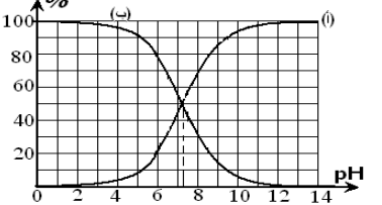
\includegraphics[width=0.34\textwidth]{./img/ex_05.png}
  \end{center}
\end{wrapfigure}
	L’acide hypochloreux a pour formule $HClO_{(aq)}$ . Sa base conjuguée $ClO^-_{(aq)}$ est appelée ion hypochlorite. Le document ci-contre représente les pourcentages des espèces chimiques acide et base du couple $HClO_{aq}/ClO^-_{(aq)}$ en fonction du $pH$ pour une solution

	\textbf{1. }Déterminer graphiquement la valeur numérique de la constante $pK_A$ du couple $HClO_{aq}/ClO^-_{(aq)}$

	\textbf{2. }Laquelle des deux courbes (a) ou (b) correspond à l'hypochlorite? Montre que
 $\%HClO$=$ \frac{[HClO]}{[HClO] + [ClO^-]} = \frac{1}{ 1 + 10^{pH -pK_A}}$
et $\%ClO^-$=$\frac{[ClO^-]}{[HClO] + [ClO^-]}$=$ \frac{1}{ 1 + 10^{pK_A - pH}}$

\textbf{3. }Écrire l'équation de la réaction de $HClO_{(aq)}$
avec de l'eau.

\textbf{4. }On considère une solution d'acide hypochloreux de
$pH=5$ . Déterminer le taux d’avancement de la réaction
dans la solution .
\end{Box2}

\end{document}
